\section{Kiting}
\label{kiting}

Kiting behavior is worth more explanation. 
We based our algorithm on the work of \cite{kiting}. 

\begin{definition}[Kiting]
    Kiting (to kite) is to move units around to make the enemy chase them and thus not be able to attack as much, or not at all. 
    Kiting can be summarize as:
    \begin{shortitem}
    \item Move out of range
    \item Turn back and shoot at the enemy
    \item Repeat
    \end{shortitem}
\end{definition}

The behavior tree used by the units achieving \texttt{Kiting} is depicted in Figure \ref{behaAttackClos}.

\begin{figure}[h!t]
\centering
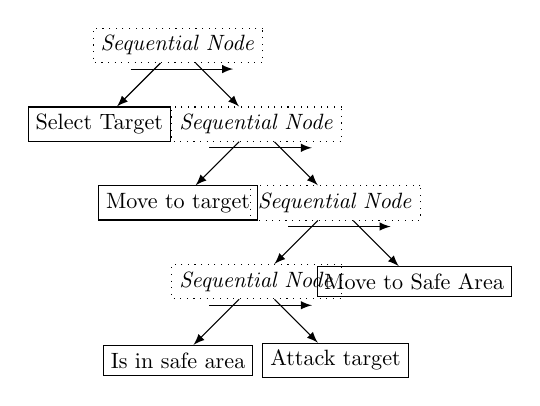
\begin{tikzpicture}[node distance = 1 cm]
    \tikzstyle{leaf}=[rectangle, align=center, scale=0.8, draw]
    \tikzstyle{node}=[rectangle,dotted, align=center, scale=0.8, draw]
    \tikzstyle{tt}=[rectangle,scale=0.8, align=center]
    \tikzstyle{link}=[->,thin,>=latex]
    \node[node] (start) at (1,4) {\emph{Sequential Node}};
    \node[tt] (start1) at (0.3,3.7) {};
    \node[tt] (end1) at (1.8,3.7) {};
    \draw[link] (start1)--(end1);

    \node[leaf] (target) at (0,3) {Select Target};

    \node[node] (seqNode) at (2,3) {\emph{Sequential Node}};
    \node[tt] (start2) at (1.3,2.7) {};
    \node[tt] (end2) at (2.8,2.7) {};
    \draw[link] (start2)--(end2);

    \node[leaf] (leafMove) at (1,2) {Move to target};
    \node[node] (seqAttack) at (3,2) {\emph{Sequential Node}};
    \node[tt] (start3) at (2.3,1.7) {};
    \node[tt] (end3) at (3.8,1.7) {};
    \draw[link] (start3)--(end3);

    \node[node] (attackNode) at (2,1) {\emph{Sequential Node}};
    \node[tt] (start4) at (1.3,0.7) {};
    \node[tt] (end4) at (2.8,0.7) {};
    \draw[link] (start4)--(end4);

    \node[leaf] (moveSafe) at (4,1) {Move to Safe Area};

    \node[leaf] (isSafe) at (1,0) {Is in safe area};
    \node[leaf] (attack) at (3,0) {Attack target};

    \draw[link] (start)--(target);
    \draw[link] (start)--(seqNode);

    \draw[link] (seqNode)--(leafMove);
    \draw[link] (seqNode)--(seqAttack);

    \draw[link] (seqAttack)--(attackNode);
    \draw[link] (seqAttack)--(moveSafe);

    \draw[link] (attackNode)--(attack);
    \draw[link] (attackNode)--(isSafe);
\end{tikzpicture}
\caption{Behavior tree for kiting}
\label{behaAttackClos}
\end{figure}

When selecting the target our bot try to select a target on which a kiting strategy can be used (for instance unit \texttt{A} can not kite another unit \texttt{A}). 
If it can not find any kitable unit then a classic attack is perform (\emph{fight to the death while standing on your position}).

As in paper \cite{kiting} the kiting bot uses an influence map for performing kiting: a 2D matrix $I_{enemy}$.

Let $e$ be an enemy. $e$ has an influence of the area $(i,j)$ of the map if the area can be reached by the enemy before performing kiting.
This relation is denoted $e \textasciitilde (i,j)$.

\begin{multline*}
    e \textasciitilde (i,j) \Leftrightarrow \\ d(e,(i,j)) \leq e.attackRange + e.speed * kitingTime
\end{multline*}

Then the influence matrix is define as:
$$
I_{enemy}(i,j) = \sum_{e \textasciitilde (i,j)}e.DPF \text{ where } DPF = \frac{e.damage}{e.cooldown}  
$$

(DPF is the damage per frame --  average damage of an unit.)

Using this matrix each unit can compute its closest safe position.
Then an attack is performed each time the unit is in a safe area.
Figure \ref{influenceMatrix} shows the influence matrix of a group of 3 units.

\begin{center}
    \begin{figure}[h!t]
        \centering
        \includegraphics[width=0.4\columnwidth]{fig/InfluenceMap.ps}
        \caption{Influence matrix created by a group of 3 units \\ 
        Darker grey means bigger threat}
        \label{influenceMatrix}
    \end{figure}
\end{center}

